\documentclass[a4paper, 11pt]{article}
\usepackage{graphicx}
\usepackage{amsmath}
\usepackage[pdftex]{hyperref}
\usepackage{subcaption}

% Lengths and indenting
\setlength{\textwidth}{16.5cm}
\setlength{\marginparwidth}{1.5cm}
\setlength{\parindent}{0cm}
\setlength{\parskip}{0.15cm}
\setlength{\textheight}{22cm}
\setlength{\oddsidemargin}{0cm}
\setlength{\evensidemargin}{\oddsidemargin}
\setlength{\topmargin}{0cm}
\setlength{\headheight}{0cm}
\setlength{\headsep}{0cm}

\renewcommand{\familydefault}{\sfdefault}

\title{Machine Learning 2015: Project 2 - Classification Report}
\author{jo@student.ethz.ch\\ sakhadov@student.ethz.ch\\ kevinlu@student.ethz.ch\\}
\date{\today}

\begin{document}
\maketitle

\section*{Experimental Protocol}
We used split-training (train on 80\%, test on 20\%) and ten fold cross-validation to select the best models. \\
To better understand the data and feature importance, we used two different plotting methods. Firstly, we plotted every combination of two features and the class on the third axis. With this we could see that there are some outliers in the data, and we could set the thresholds for the outliers visually. From figure \ref{2Features} we can see that we can set the threshold to 4 on the frequency 1, because the points beyond this limit are clearly to far away from the centers.\\ 
Furthermore, we plotted all combinations of three features on a 3D graph. With this technique we could examine the importance of each feature. Figure \ref{3Features} shows that the frequency 5 has probably no impact on the labels, because the means of different classes lay roughly on the same height. \\
We tried different classification algorithms including Random Forests and SVM. The best result was achieved with gradient boosting library xgboost. \\
To also make use of the available validation data, we trained Gaussian Mixture Models to create additional feature vector with its predicted labels. The labels where then binarized and added to the training data.



\begin{figure}[!b!]
 \centering 
\begin{subfigure}[b]{0.4\textwidth}
	\centering
	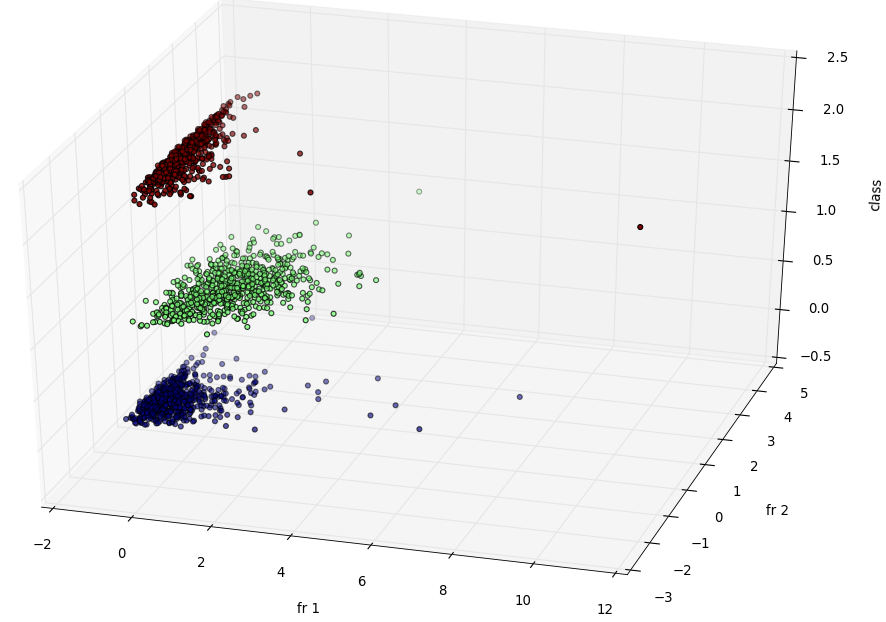
\includegraphics[width=\textwidth]{2_features.png} 
	\caption{There are several outliers which can be detected visually. On the fr 1 axis we can set every point greater then 4 to be an outlier.}
	\label{2Features}
\end{subfigure}
\hfill
\begin{subfigure}[b]{0.4\textwidth}
	\centering
	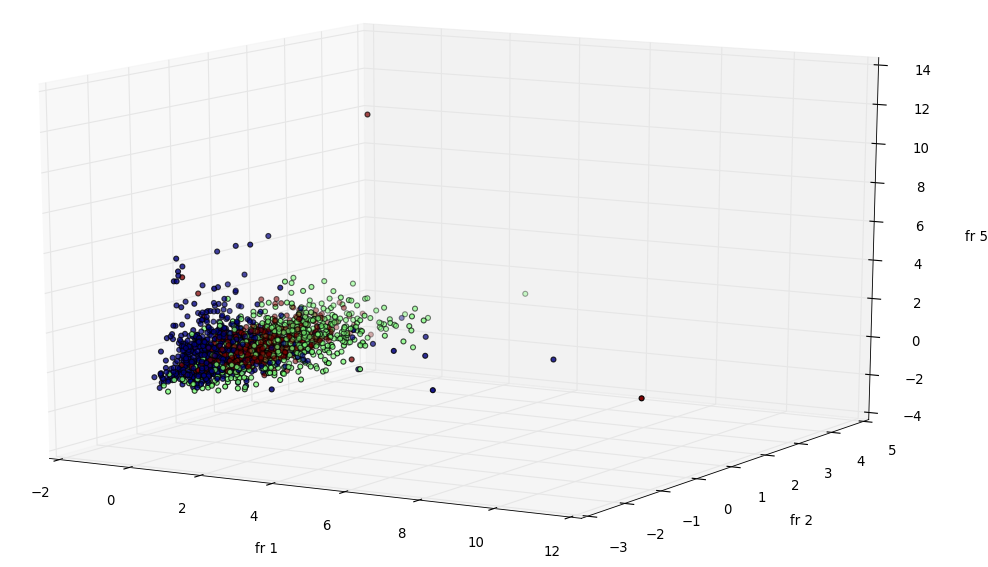
\includegraphics[width=\textwidth]{3_features.png} 
	\caption{The vertical axis does not differentiate well between different classes. The bulk of the three classes lays roughly on the same height, rendering frequency 5 useless for learning.}
	\label{3Features}
\end{subfigure}
\caption{We used different visualization strategies to better understand the data. On the left two different features are plotted on the horizontal axis and the labels on the vertical axis. On the right three different features are plotted on three axis and the data points have the color of its class.}
\end{figure}

\section{Tools}
We used Python 2 with the machine learning library \textit{scikit-learn} and \textit{numpy}. For Gradient Boosting we used XGBoost python library.

\section{Algorithm}
We first normalize all the features and delete random feature frequency 5. Then we use Gaussian Mixture Model to make predictions on the labels, binarize them and add as feature vectors to our training data. To train GMM we use all the available data in semi-supervised fashion. To initialize the means of the GMM we use the means computed from the training data. During the training we allow GMM algorithm to adjust the means which results in a worse training data performance but is better for generalisation. \\
The resulted features are used to train the XGBoost classifier. 

\section{Features}
We deleted the feature with no importance fr 5 and added the labels predicted by the GMM as the new features.

\section{Parameters}
Parameters were found using grid search. For every possible set of parameters 10-fold cross-validation was performed to find the best generalizing parameters. To validate the model afterwards, a 10-fold cross-validation was applied together with a split-test, where we trained on 80\% of the data and tested on the other 20\%.

\section{Lessons Learned} Data visualization plays an important role in machine learning.

\end{document}
